\documentclass[12pt,letterpaper]{article}
\usepackage{graphicx,textcomp}
\usepackage{natbib}
\usepackage{setspace}
\usepackage{fullpage}
\usepackage{color}
\usepackage[reqno]{amsmath}
\usepackage{amsthm}
\usepackage{fancyvrb}
\usepackage{amssymb,enumerate}
\usepackage[all]{xy}
\usepackage{endnotes}
\usepackage{lscape}
\newtheorem{com}{Comment}
\usepackage{float}
\usepackage{hyperref}
\newtheorem{lem} {Lemma}
\newtheorem{prop}{Proposition}
\newtheorem{thm}{Theorem}
\newtheorem{defn}{Definition}
\newtheorem{cor}{Corollary}
\newtheorem{obs}{Observation}
\usepackage[compact]{titlesec}
\usepackage{dcolumn}
\usepackage{tikz}
\usetikzlibrary{arrows}
\usepackage{multirow}
\usepackage{xcolor}
\newcolumntype{.}{D{.}{.}{-1}}
\newcolumntype{d}[1]{D{.}{.}{#1}}
\definecolor{light-gray}{gray}{0.65}
\usepackage{url}
\usepackage{listings}
\usepackage{color}

\definecolor{codegreen}{rgb}{0,0.6,0}
\definecolor{codegray}{rgb}{0.5,0.5,0.5}
\definecolor{codepurple}{rgb}{0.58,0,0.82}
\definecolor{backcolour}{rgb}{0.95,0.95,0.92}

\lstdefinestyle{mystyle}{
	backgroundcolor=\color{backcolour},   
	commentstyle=\color{codegreen},
	keywordstyle=\color{magenta},
	numberstyle=\tiny\color{codegray},
	stringstyle=\color{codepurple},
	basicstyle=\footnotesize,
	breakatwhitespace=false,         
	breaklines=true,                 
	captionpos=b,                    
	keepspaces=true,                 
	numbers=left,                    
	numbersep=5pt,                  
	showspaces=false,                
	showstringspaces=false,
	showtabs=false,                  
	tabsize=2
}
\lstset{style=mystyle}
\newcommand{\Sref}[1]{Section~\ref{#1}}
\newtheorem{hyp}{Hypothesis}

\title{Problem Set 5}
\date{Due: March 4, 2020}
\author{QTM 200: Applied Regression Analysis}

\begin{document}
	\maketitle
	
	\section*{Instructions}
	\begin{itemize}
		\item Please show your work! You may lose points by simply writing in the answer. If the problem requires you to execute commands in \texttt{R}, please include the code you used to get your answers. Please also include the \texttt{.R} file that contains your code. If you are not sure if work needs to be shown for a particular problem, please ask.
		\item Your homework should be submitted electronically on the course GitHub page in \texttt{.pdf} form.
		\item This problem set is due at the beginning of class on Wednesday, March 4, 2020. No late assignments will be accepted.
		\item Total available points for this homework is 100.
	\end{itemize}
	
		\vspace{.5cm}
	
\noindent  Using the \texttt{teengamb} dataset, fit a model with \texttt{gamble} as the response and the other variables as predictors. 

\vspace{.5cm}
\lstinputlisting[language=R, firstline=41, lastline=43]{PS5.R}  
\vspace{.5cm}
Answer the following questions:
\vspace{.5cm}
\begin{enumerate}[(a)]
	 \item Check the constant variance assumption for the errors by plotting the residuals versus the fitted values.
\lstinputlisting[language=R, firstline=45, lastline=54]{PS5_answers.R}
\begin{figure}
	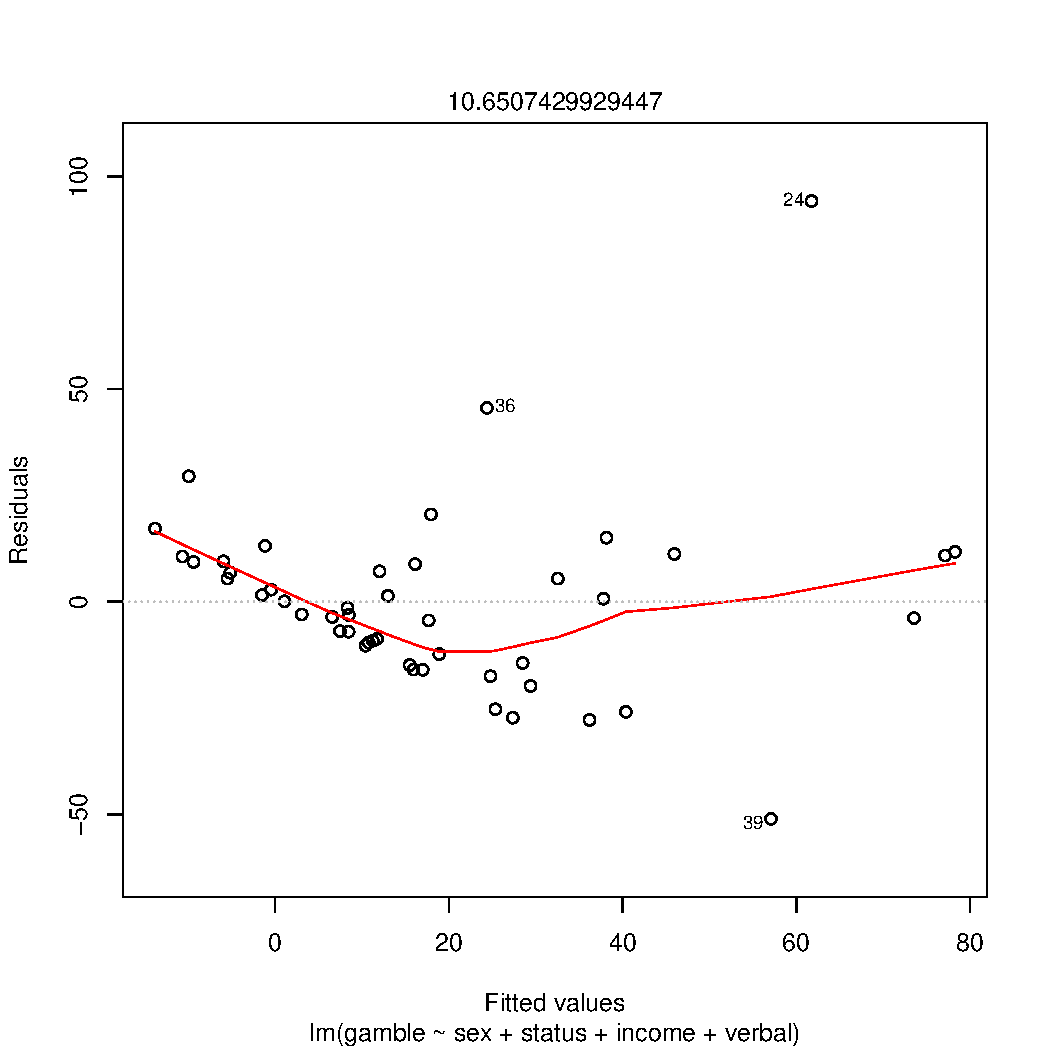
\includegraphics[width=.5]{ResidFVplot.pdf}
	\end{figure}
	 
	  \newpage
	\item Check the normality assumption with a Q-Q plot of the studentized residuals. \vspace{1cm}
\lstinputlisting[language=R, firstline=56, lastline=63]{PS5_answers.R}
\begin{figure}
	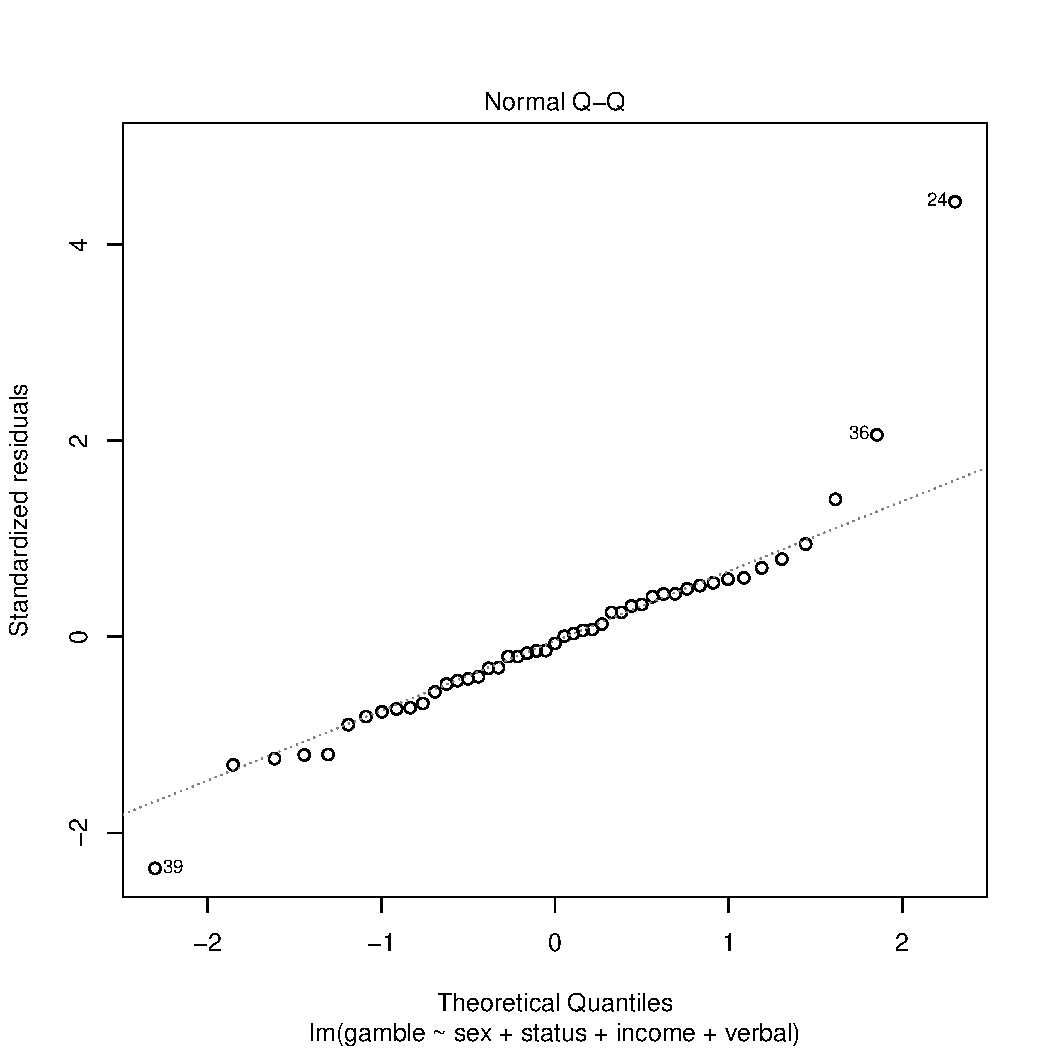
\includegraphics[width=.5]{QQplot.pdf}\\
	\end{figure}
	\item Check for large leverage points by plotting the $h$ values. \vspace{1cm}
\lstinputlisting[language=R, firstline=65, lastline=77]{PS5_answers.R}
\begin{figure}
	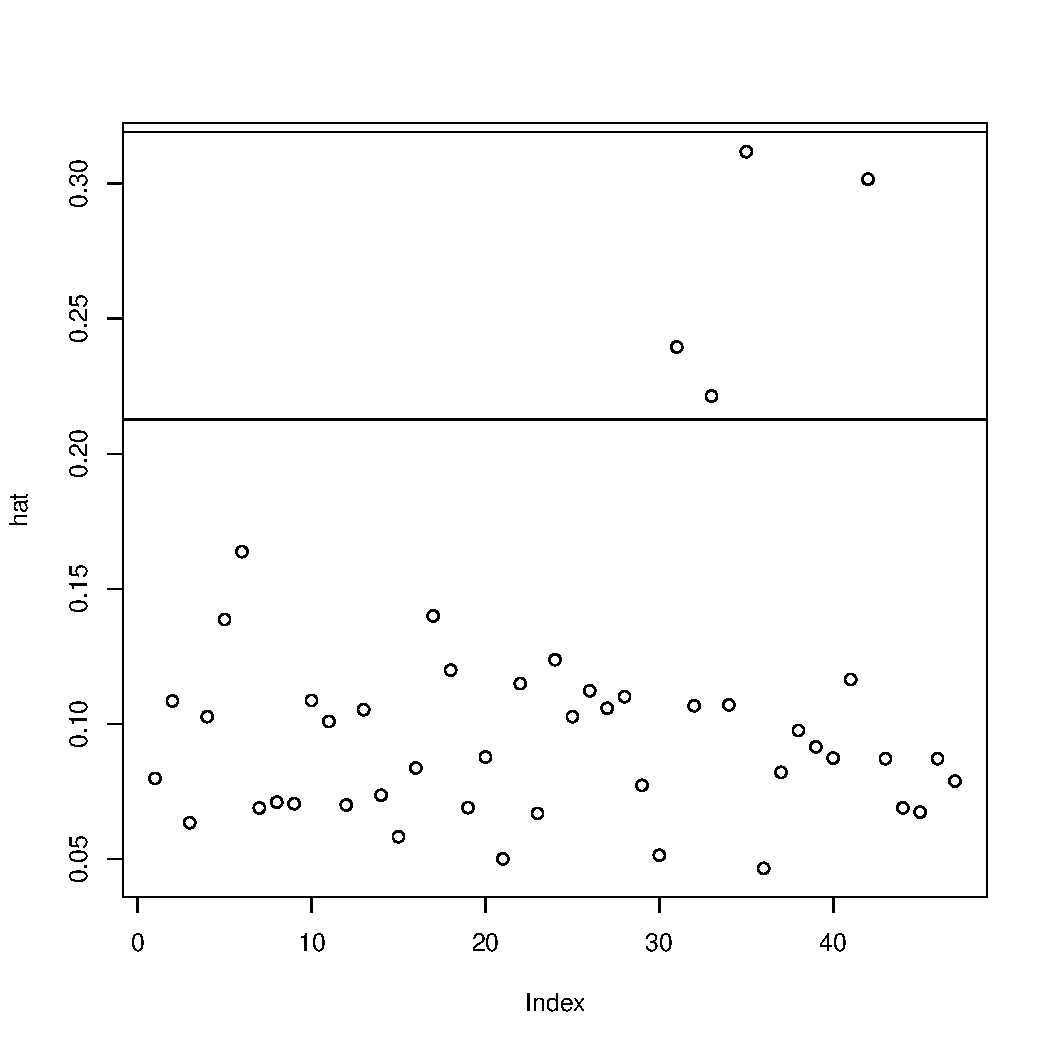
\includegraphics[width=.5]{hvalueplot.pdf}\\
	\end{figure}
	\item Check for outliers by running an \texttt{outlierTest}. \vspace{1cm}
\lstinputlisting[language=R, firstline=79, lastline=81]{PS5_answers.R}
	\item Check for influential points by creating a "Bubble plot" with the hat-values and studentized residuals.
\lstinputlisting[language=R, firstline=83, lastline=95]{PS5_answers.R}
\begin{figure}
	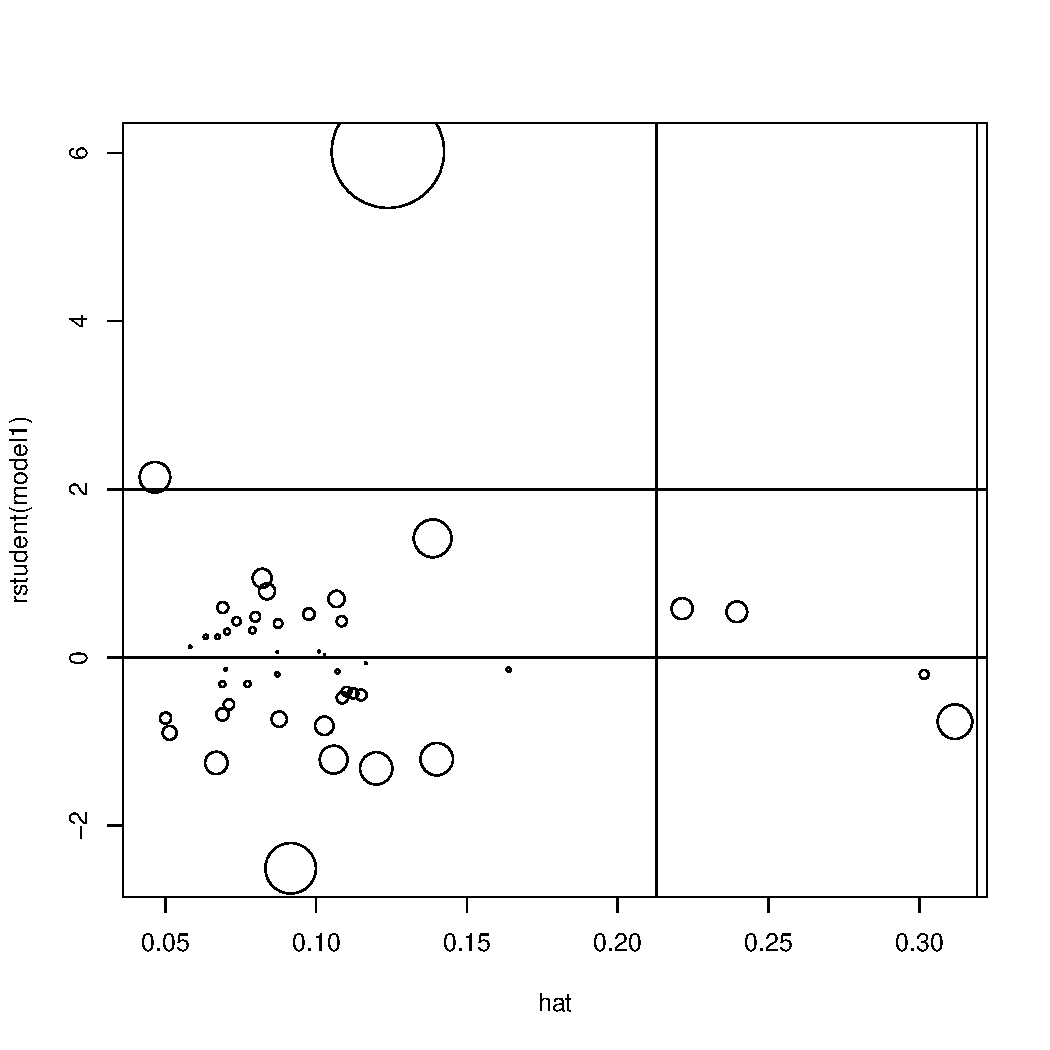
\includegraphics[width=.5]{bubbleplot.pdf}\\
	\end{figure}
	% \item N/A.
\end{enumerate}

\end{document}
